\documentclass[11pt,a4paper]{scrartcl}
%\documentclass[11pt,a4paper]{article}

\usepackage[affil-it]{authblk}
\usepackage{geometry}
\geometry{
    a4paper, 
    total = {140mm, 230mm}, 
    left = 22mm, 
    top = 30mm, 
    marginparsep = 1cm,    % distance between text body and margin note
    marginparwidth = 3cm   % width of margin note
}
\usepackage{marginnote}
\usepackage{url}
\usepackage{natbib}
%\usepackage{libertine}
\usepackage{pgfgantt}
\usepackage{pdflscape}


% The title of your topic should be succinct.
% Less than 15 words is the rule of thumb.
\title{

\includegraphics[height=5cm,width=0.8\textwidth]{WSU.PNG}\\
Is the FIFA World Cup Draw Truly Random?}
\author{Pratik Kulkarni (19400570)\\ Shrey Parekh (18706941)}
\affil{Project proposal for 301111 Discovery Project}
\author{Supervisor: Dr Russell Thompson}

% A project proposal submitted for \@unitnumber{} \@unitname{}
% in partial fulfilment of the requirements for the degree of
% \@degree{}. 
% Supervisor: \@supervisor{}

\affil{School of Computer, Data and Mathematical Sciences, \\ Western Sydney University}

\date{Spring, 2021}

\setcounter{tocdepth}{2}



\begin{document}


\maketitle

% This proposal document is the starting point and will gradually evolve
% into the final progress report for this unit and the final report for
% the subsequent unit.

\newpage

\renewcommand\contentsname{Table of Contents}

\tableofcontents

\newpage

\section{Background}

\marginnote{This section is written by Pratik Kulkarni (19400570) }

Is the FIFA World Cup draw truly random?
\\ \\
This is the topic chosen for our Discovery Project. The topic was selected by our supervisor, Dr Thompson while watching a soccer match and decided to investigate this topic.
We intend to investigate whether the FIFA World Cup draw is truly random and if each group has an even chance of being drafted into the groups. 
\\ \\
Researchers such as \citet{cea2020analytics}, conducted research on a similar topic. In this paper, they found that one of those main factors that affects the countries chances of being drafted is their home-away status. While this does not directly affect the team ranking by points, a general belief is that teams always play better at home, this factor has not yet been considered in the draw of teams so far. This affects their game due to the home team feeling stronger with a crowd that is supportive of them. This in turn influences their world ranking. Moreover, another factor found in this paper’s research was that until the 2018 World Cup, teams would avoid friendly games due to friendlies awarding very few points, teams that would play more friendlies had less chances of going further up the team ranking table as compared to teams who avoided friendly matches and climbed up the ranks. 
\\ \\
In the 2018 World Cup, FIFA changed the draw system to a rank-based system, the groups would be split by the team’s rankings. While this could be a better system, there are chances that the groups might become unbalanced, especially if a low ranked host country was placed in the top group with the best teams.
\\ \\
The knowledge gap in this topic would be that there is no fairness index created by any researchers. To fill this gap, we would have to make a fairness index for each team that did qualify for our chosen year of the world cup based on their FIFA team ranking in the same groups.


\section{Objective}

\marginnote{This section is written by Shrey Parekh (18706941) }

The Supervisors goals are centred on providing value and results to the fans. This can be seen through testing the randomness of the FIFA world cup draw. The goal of this project is to determine the predictions of the simulated world cup draw. Aim is to discover the fairness index for each team that qualified for the world cup, based on the FIFA team rankings of the teams in the same grouping. This will allow us to determine that world cup draw is based on chance or is done through an algorithm.
\\ \\
We will establish whether the fairness index affects the performance through multiple linear regression or non-parametric tests. This will increase the scope of this project as we will be able to produce efficient statistical results to ascertain the influences of chance in the FIFA world cup draw.
\\ \\
This can be further reinforced by simulating the world cup draws to test if any countries have a fairness index that is higher or lower than expected by chance alone.  This is to proclaim that certain countries will not have a favourable advantage while competing in the world cup.


\section{Hypothesis/question}

\marginnote{This section is written by Shrey Parekh (18706941) }

Is the FIFA world cup draw truly random? 
               	
\subsection{Why Ask this Question? }

This is a concern fueled by the excitement of the fans of FIFA world cup. This is important because it raises an interest about who will win this year’s trophy. It also generates a doubt in the mind of the fans if the draw of the teams competing against each other is a fair competition, or is it based on chance. They want to know the algorithm that is used to decide the matchups of the team.
\\ \\
The value of answering this question is that it will remove the doubts from people’s minds. This will allow the fans to determine that the teams competing are fairly matched up. They will be able to then ascertain that the draws are random, and each team is given a fair chance to progress through the tournament. This will provide confidence for fans as the best performing team will win not any team based on chance.

\subsection{Data Question}

Can we predict accurately the winning team of the FIFA World Cup?

\subsection{Data}

The data is sourced from the supervisor.

\newpage

\subsection{Data Science Process}

\subsubsection{Data Analysis}

The Data pipeline that was used to wrangle the raw data is below:
\\ \\
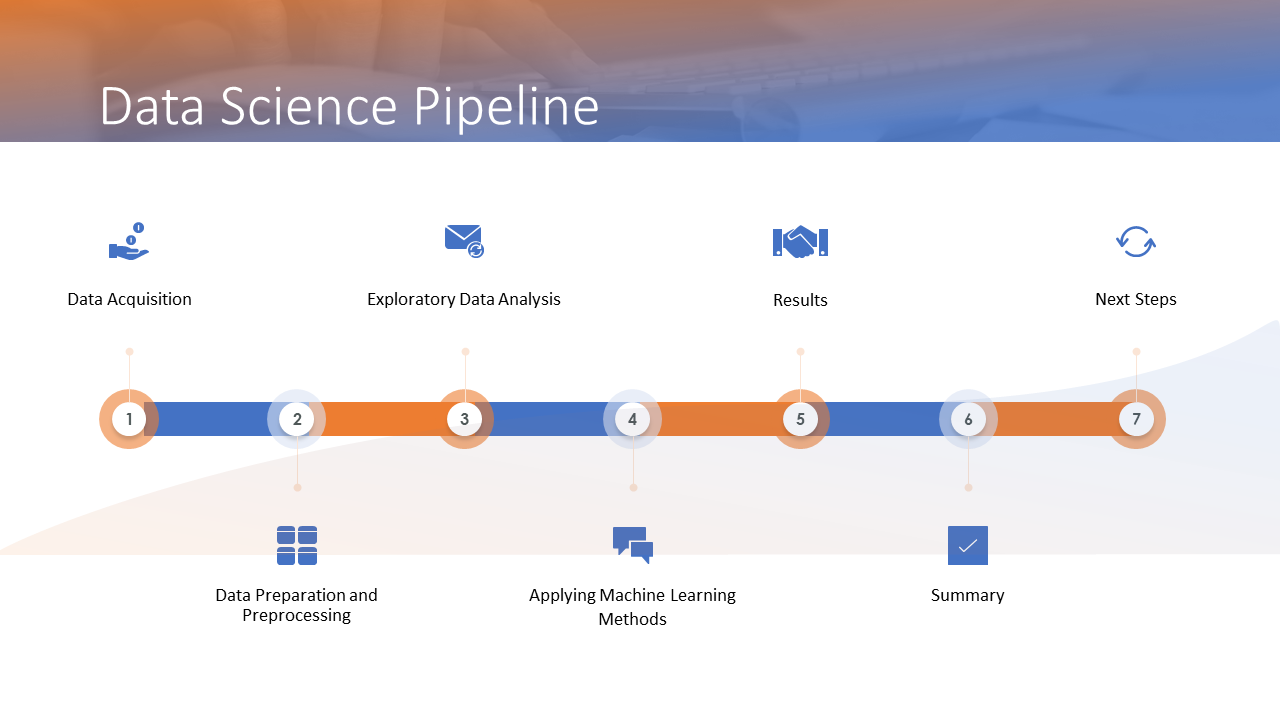
\includegraphics[height=7.5cm,width=\linewidth]{datascipipeline.PNG}


\section{Methodology}

\marginnote{This section is written by Shrey Parekh (18706941) }

The goal of our project is to create a fairness index for each team that qualified for the world cup based on team rankings. Test the performance being affected by index through multiple linear regression tests and non-parametric tests. Simulating the world cup draw to observe the draws are fair and not based on chance.
\\ \\
The steps to obtain results in this project required are:


\begin{enumerate}
\item Data gathering from the supervisor data was obtained that consisted of FIFA world cup matches from 1992 to 2021. The team needs to source another data set or will have to scrape data manually to get the rankings and merge it with the current data set. The two data sets will need to be merged.
\item The next step consists of performing feature engineering that will allow us to predict the best team of winning the FIFA world cup.
\item Exploratory Data Analysis on the data set to obtain insights from the world cup data.
\item Data preparation and pre-processing the data will be cleaned to filter out any missing data, corrupted data from the data set. This will enable the team to get accurate results in predicting the winning team.
\item Then machine learning models will be applied to the data set
	\begin{itemize}
	\item Splitting the data set in proportions to 80 to 20 ratio.
	\item Then will performing normalization
	\item Building the models
	\item Then we will predict the winning team
	\item Plot the ROC curve
	\end{itemize}
\end{enumerate}

\subsection{Block Diagram}
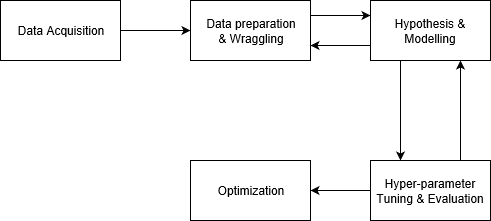
\includegraphics[height=6cm,width=\linewidth]{methodflow.PNG}


\section{Expected outcomes}

\marginnote{This section is written by Pratik Kulkarni (19400570) }

The expected outcome at the end of this project would be to gain a deeper understanding of the topic. Another outcome would be discovering any trends from gathering data of previous FIFA team rankings, seeing if there are any common reoccurring factors. Assuming the draw is not ‘truly random’, we also hope to find out if there are any factors that would give some teams a higher chance of being drafted for the World Cup. 

\newpage

\section{Program of work}

\marginnote{This section is written by Pratik Kulkarni (19400570) }

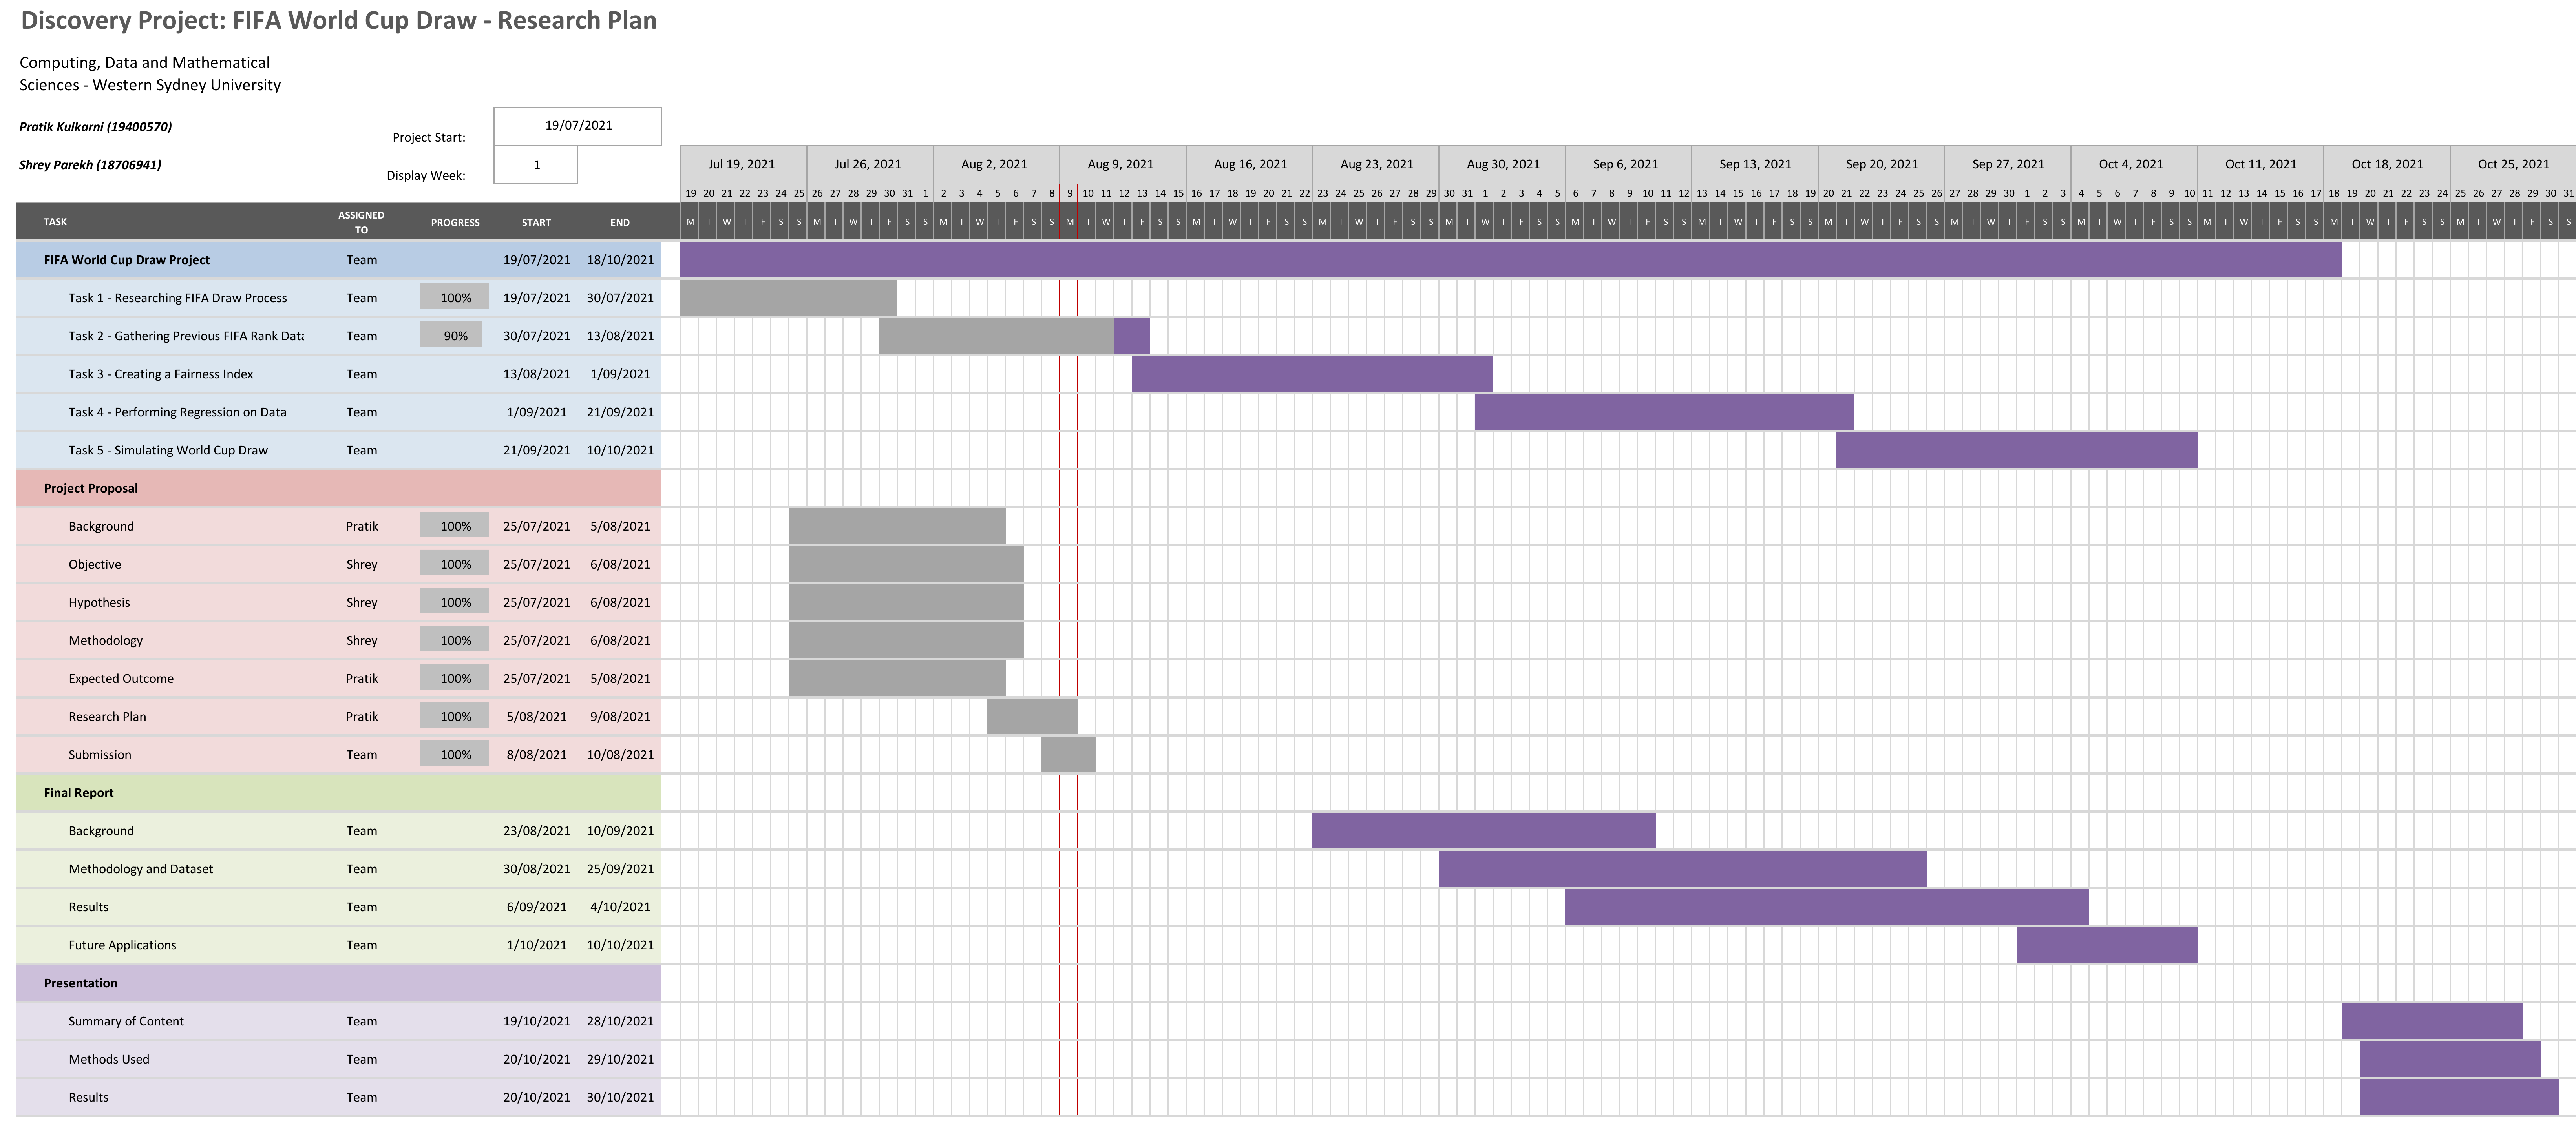
\includegraphics[angle=90,height=20cm,width=\linewidth]{ProposalGantt.PNG}


\newpage

\bibliographystyle{plainnat}
\bibliography{project}

\end{document}

%%% Local Variables:
%%% mode: latex
%%% TeX-master: t
%%% End:
